\documentclass[12pt]{article}
\usepackage{amsmath}
\usepackage[margin = 1in]{geometry}
\usepackage{graphicx}
\usepackage{booktabs}
\usepackage{natbib}
% highlighting hyper links
\usepackage[colorlinks=true, citecolor=blue]{hyperref}

%% meta data
\title{Data analytics effects in Baseball}
\author{Chenyu Mu\\
  Department of Statistics\\
  University of Connecticut
}

\begin{document}

\maketitle

\begin{abstract}
  Over the past two decades, there has been a notable resurgence in the utilization of data analytics across professional sports, businesses, and governmental sectors.
  This article will delve into an in-depth analysis of the myriad factors that potentially impact baseball players while they are actively engaged in the game. 
  The study aims to explore and elucidate the diverse elements that might influence and shape the performance, strategies, and outcomes within the realm of baseball. 
  \end{abstract}


\section{Introduction}
\label{sec:intro}
Sport psychology, an interdisciplinary field integrating concepts from both psychology and sports science, has become a fundamental element in enhancing athletic performance across a spectrum of sports, baseball included.
Its primary focus is to comprehend and optimize the psychological components that affect an athlete's mindset, emotions, and conduct, ultimately aiming to elevate their performance.
Now, let's explore specific key domains within sport psychology that exert significant influence on baseball players.
Baseball was selected as the focal sport due to its comprehensive nature, allowing for an analysis of nearly every facet of the game, except for the mental readiness of the player upon entering the field. 
Previous studies in the field \cite{Dalmass2018baseball} have provided valuable insights, and we seek to build upon their findings. 

We measure performance in these two dimensions: 
\begin{enumerate}
\item the player's subjective assessment of their performance. 
\item the statistical analysis of the player's actual performance. Consequently, the research inquiries encompass the following:
\end{enumerate}
\begin{itemize}
  \item Does sports psychology have an effect on a player's physical performance?
  \item Does sports psychology have an effect on the way a player feels about his performance?
  \item Can sports psychology be used to ensure that a player is almost always giving his best performance?
\end{itemize}

% roadmap
The rest of the paper is organized as follows.\\
The data will be presented in Section~\ref{sec:data}.\\
The methods are described in Section~\ref{sec:meth}.\\
The results are reported in Section~\ref{sec:resu}.\\
A discussion concludes in Section~\ref{sec:disc}.\\


\section{Data}
\label{sec:data}
Following are definitions we may use:\\
$AB$: At bats\\ 
$AVG$: Batting average\\ 
$H$: Hits\\
$K$: Killed,Strikeout \\
$HR$: Home Run\\
$BABIP$: Batting Average on Balls in Play\\
$SF$: sacrifice flies\\
\begin{equation}
  \label{eq:AVG}
  AVG = H/AB,
\end{equation}
which means the total number of hits divided by the total number of at-bats
\begin{equation}
  \label{eq:BABIP}
  BABIP = (H - HR) / (AB - K - HR - SF),
\end{equation}
which states that a batter's average for balls that are put in play (excludes strikeouts, home runs, and sacrifice flies)


We can see the number of players in each team in Figure~\ref{fig:team}.
\graphicspath{{images/}}

\begin{figure}[tbp]
  \centering
  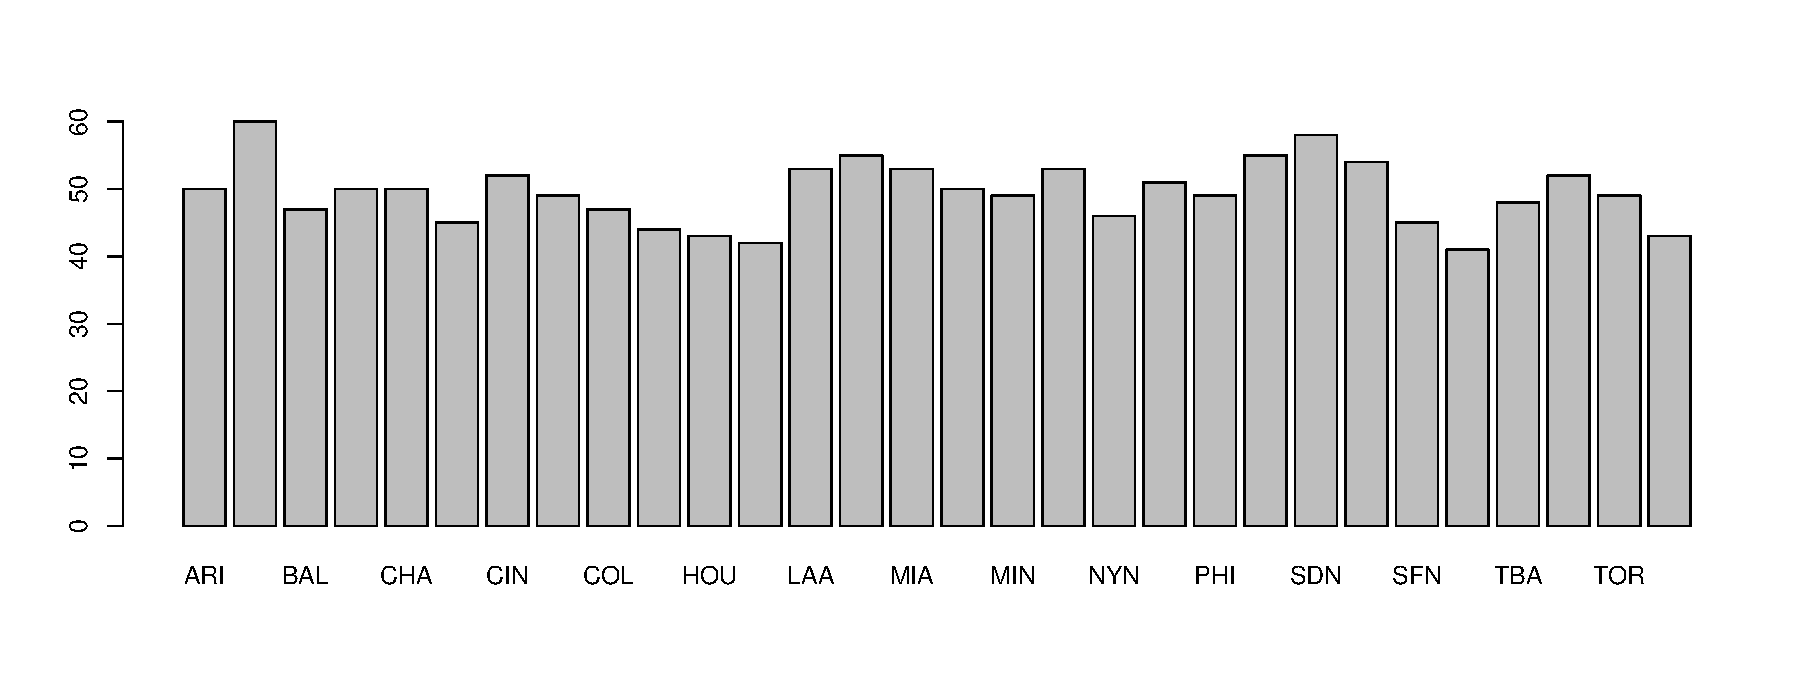
\includegraphics[width=\textwidth]{baseball team.pdf}
  \caption{The number of players in each team in 2016 batting dataset}
  \label{fig:team}
\end{figure}

\section{Methods}
\label{sec:meth}
The research was structured as a two-sample experiment utilizing a differences-in-differences analysis method.
The participants were classified into three positional groups and then subdivided into either control or experimental groups. 
The outcomes were assessed using t-tests to analyze the differences in means between the groups.Method way\cite*{Dalmass2018baseball}.




\section{Results}
\label{sec:resu}
These limitations encompassed various factors, including but not restricted to the sample size, the participants' in-season playing time,
and the number of at-bats and innings pitched. The relatively small sample size utilized in the study, which significantly impacted the practicality of the results.

\begin{table}[tbp]
  \caption{The distribution of censored participants}
  \label{tab:rv}
\centering
\begin{tabular}{rrrr}
  \toprule
  Position & Assigned Group & Did Not Meet AB or IP & Did Not Play\\ 
  \midrule
Pitcher & Control & 3 & 1\\
Pitcher & Experiment & 2 & 1\\
Infield & Control & 1 & 0 \\
Infield & Experiment & 2 & 2\\
Outfield & Control & 1 & 0\\
Outfield & Experiment & 1 & 0\\
  \bottomrule
\end{tabular}
\end{table}

\section{Discussion}
\label{sec:disc}




\begin{thebibliography}{9}

  \bibliography{refs.bib}
  \bibliographystyle{chicago}
\end{thebibliography}

\end{document}